\documentclass[paper=a4, fontsize=13pt]{scrartcl} % A4 paper and 11pt font size
\renewcommand{\baselinestretch}{1.5}

\usepackage[utf8]{inputenc}
\usepackage[T1, T2A]{fontenc}
\usepackage[russian]{babel}
\usepackage{amsmath,amsfonts,amsthm} % Math packages

\usepackage{bm}

\usepackage{sectsty} % Allows customizing section commands
\allsectionsfont{\centering \normalfont\scshape} % Make all sections centered, the default font and small caps

\usepackage{graphicx}
\graphicspath{ {images/} }

\usepackage{fancyhdr} % Custom headers and footers
\pagestyle{fancyplain} % Makes all pages in the document conform to the custom headers and footers
\fancyhead{} % No page header - if you want one, create it in the same way as the footers below
\fancyfoot[L]{} % Empty left footer
\fancyfoot[C]{} % Empty center footer
\fancyfoot[R]{\thepage} % Page numbering for right footer
\renewcommand{\headrulewidth}{0pt} % Remove header underlines
\renewcommand{\footrulewidth}{0pt} % Remove footer underlines
\setlength{\headheight}{13.6pt} % Customize the height of the header

\numberwithin{equation}{section} % Number equations within sections (i.e. 1.1, 1.2, 2.1, 2.2 instead of 1, 2, 3, 4)
\numberwithin{figure}{section} % Number figures within sections (i.e. 1.1, 1.2, 2.1, 2.2 instead of 1, 2, 3, 4)
\numberwithin{table}{section} % Number tables within sections (i.e. 1.1, 1.2, 2.1, 2.2 instead of 1, 2, 3, 4)

\setlength\parindent{0pt} % Removes all indentation from paragraphs - comment this line for an assignment with lots of text

%----------------------------------------------------------------------------------------
%	TITLE SECTION
%----------------------------------------------------------------------------------------

\newcommand{\horrule}[1]{\rule{\linewidth}{#1}} % Create horizontal rule command with 1 argument of height

\title{
\normalfont \normalsize
\textsc{Московский государственный университет имени М. В. Ломоносова} \\ [25pt] % Your university, school and/or department name(s)
\horrule{0.5pt} \\[0.4cm] % Thin top horizontal rule
\huge Решение уравнения теплопроводности на квадратной пластинке методом конечных элементов  \\ % The assignment title
\horrule{2pt} \\[0.5cm] % Thick bottom horizontal rule
}

\author{Карпенко Виталий \\
424 группа} % Your name

\date{\normalsize\today} % Today's date or a custom date

\begin{document}

\maketitle % Print the title
\newpage
\section{Исходная дифференциальная задача}
    \[
        \begin{cases}
            u_t = \bigtriangleup_x u + f& \text{на $\Omega \times (0, \inf)$,} \\
            u(\cdot, 0) = u_0& \text{на $\Omega$}, \\
            u(\cdot, 0) = g& \text{на $\Gamma$ для $\forall t > 0$,}
        \end{cases}
    \]
Здесь $\Omega$ - квадратная область в плоскости $(x, y)$ с левым нижним углом в $(0, 0)$ и правым верхним в $(1, 1)$.
$\Gamma$ - граница пластинки. Отсчёт времени начинается в $t_0 = 0$. Необходимо найти $u(\bm{x}, t) = u(x, y, t)$.
\section{Дискретизация}
\subsection{Дискретизация по времени и задача в слабой форме}
Разбиение по времени может быть произвольным $0 = t_0 < t_1 < t_2 < ... < t_n < ...$, но в данном случае удобнее пользоваться постоянным шагом (позже будет видно почему), хотя при необходимости метод легко модифицируется для вычисления временных шагов в зависимости от поведения численного решения или производительности метода в данный момент времени. Таким образом $\delta_n = t_{n+1} - t_n = const$.
При этом $f_n = f(\cdot, t_n) : \Omega \rightarrow \mathbb{R}$, $g_n = g(\cdot, t_n) : \Omega \rightarrow \mathbb{R}$.
Для аппроксимации производной $u$ по $t$ используется следующая формула $$\phi'(t_{n+1}) = \frac{\phi(t_{n+1}) - \phi(t_{n})}{t_{n+1} - t_{n}} = \frac{\phi(t_{n+1}) - \phi(t_{n})}{\delta_n}$$, т.е. в нашем случае $\frac{u_{n+1} - u_n}{\delta_n} = \bigtriangleup u_{n+1} + f_{n+1}$.
Тогда, применяя теорему Грина к $u_n$: $$\int_{\Omega}(\bigtriangleup u_n)v + \int_{\Omega}\bigtriangledown u_n \bigtriangledown v = \int_{\Gamma}(\partial_n u_n)v$$, откуда получаем формулировку задачи в слабой форме для вычисления $u_{n+1}$:
    \[
        \begin{cases}
            \text{найти } u_{n+1} \in H^1(\Omega)\text{, такую, что:} \\
            u_{n+1} = g_{n+1}& \text{на $\Gamma$,} \\
            \delta_n \int_{\Omega} \bigtriangledown u_{n+1} \bigtriangledown v + \int_{\Omega} u_{n+1}v = \int_{\Omega} u_{n}v + \delta_n \int_{\Omega} f_{n}v& \forall v \in H^1_0(\Omega).
        \end{cases}
    \]
\subsection{Дискретизация по пространству}
Данная квадратная пластинка разбивается на треугольники, имеющие в пересечениях только общие вершины или общие рёбра.
Используется самая простая вариация метода конечных элементов с треугольными элементами первой степени, сетка выглядит, например, так: \\
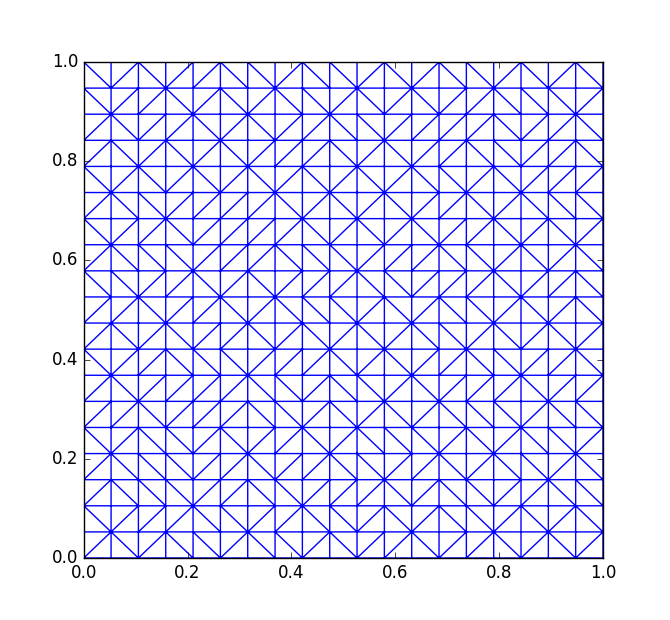
\includegraphics[scale=0.5]{mesh} \\
Мы имеем пространство функций $V_h \in H^1(\Omega)$ определяемых значениями в узлах триангуляции, узлы разбиения, узлы с граничными условиями Дирихле (все граничные в данном случае) и подпространство $$V^0_h = V_h \cap H^1_0(\Omega) = \{v_h \in V_h | v_h = 0 \text{ на $\Gamma$.}\}$$ Узлы пронумерованы и их номера содержатся в двух списках - Dir для граничных и Ind для внутренних. Теперь мы заменяем все элементы слабой формулировки на их дискретные аналоги:
    \[
        \begin{cases}
            \text{найти } u^h_{n+1} \in V_h\text{, такую, что:} \\
            u^h_{n+1}(p_i) = g_{n+1}(p_i)& \text{для $\forall i \in Dir$,} \\
            \delta_n \int_{\Omega} \bigtriangledown u^h_{n+1} \bigtriangledown v_h + \int_{\Omega} u^h_{n+1}v_h = \int_{\Omega} u^h_{n}v_h + \delta_n \int_{\Omega} f_{n}v_h& \forall v_h \in V^0_h.
        \end{cases}
    \]
Тогда, если $W$ - матрица жёсткости, а $M$ - матрица масс, то каждый шаг решения можно записать как:
    \[
        \begin{cases}
            u^{n+1}_{Dir} = g_{n+1}, \\
            (\delta_n W + M) u^{n+1} = M u^n - f_n.
        \end{cases}
    \]
\newpage
\section{Анализ устойчивости}
Упростим задачу, положив $f$ и $g$ не зависящими от времени. Тогда:
    \[
        \begin{cases}
            u_t = \bigtriangleup_x u + f& \text{на $\Omega \times (0, \inf)$,} \\
            u(\cdot, 0) = u_0& \text{на $\Omega$}, \\
            u(\cdot, t) = g& \text{на $\Gamma$ для $\forall t > 0$,}
        \end{cases}
    \]
Если мы игнорируем начальное состояние, мы можем рассматривать только устойчивое решение задачи:
    \[
        \begin{cases}
            -\bigtriangleup u_{lim} = f& \text{на $\Omega$}, \\
            u_{lim} = g& \text{на $\Gamma$.}
        \end{cases}
    \]
Предположим теперь, что нам известны все собственные значения и собственные функции оператора Лапласа на $\Omega$:
    \[
        \begin{cases}
            -\bigtriangleup \phi_k = \lambda_k \phi_k& \text{на $\Omega$}, \\
            \phi_k = 0& \text{на $\Gamma$.}
        \end{cases}
    \]
Решение (полученное разделением переменных) $$u(\bm{x}, t) = u_{lim}(\bm{x}) + \sum_{k=1}^{\inf} c_k e^{-\lambda_k t} \phi_k(\bm{x})$$, где $c_k = \int _\Omega (u_0 - u_{lim}) \phi_k$. Эта формула показывает, что решение убывает экспоненциально быстро к устойчивому решению.

Если мы рассматриваем стремящиеся к нулю граничные условия и $f = 0$, а так же фиксированный шаг по времени, то $u^{n+1}$ получается следующим образом: $$(\delta W + M) u^{n+1} = M u^n$$ при начальном состоянии $u^0$. Если $u^0 = \phi_k$, то собственные вектора удовлетворяют уравнению $$(\delta W + M) \phi_k = (1 + \lambda_{h, k}) M \phi_k$$ Тогда легко показать, что $$u^n = (1 + \lambda_{h, k})^{-n} \phi_k$$ Т.к. $0 < (1 + \lambda_{h, k})^{-1} < 1$ метод устойчив.
\newpage
\section{Решение}
\subsection{Инструменты}
Для решения использовался язык Python и библиотеки matplotlib для построения графиков и numpy для более быстрой и удобной работы с большими объёмами численной информации.
\subsection{Проверка корректности и скорость сходимости}
Для проверки корректности решения и определения скорости сходимости исследуем следующую задачу:
$$u_t(x, y, t) = u_{xx}(x, y, t) + u_{yy}(x, y, t), t > 0, (x, y) \in [0, 1] \times [0, 1]$$
$$u(0, y, t) = 0, u(1, y, t) = 0, u(x, 0, t) = 0, u(x, 1, t) = 0$$
$$u(x, y, 0) = x(1 - x)y(1-y)$$
Аналитическое решение имеет вид (выкладки с его получением достаточно объёмны и в отчёте не приводятся):
$$u(x, y, t) = \frac{16}{\pi^6} \sum^{\inf}_{n,m=1} \frac{((-1)^n - 1)((-1)^m - 1)e^{\lambda_{n,m}t}}{n^3m^3} \sin{\pi n x} \sin{\pi m y}$$
где $\lambda_{n,m} = - \pi^2(n^2 + m^2)$. Зафиксируем момент времени $t = 1$ и сетку. Затем будем мельчить шаг по времени и смотреть, как ведёт себя норма разности численного и аналитического решений по отношению к шагу по времени. Из графика хорошо видно, что значение отношения выходит на константу - первый порядок сходимости. \\
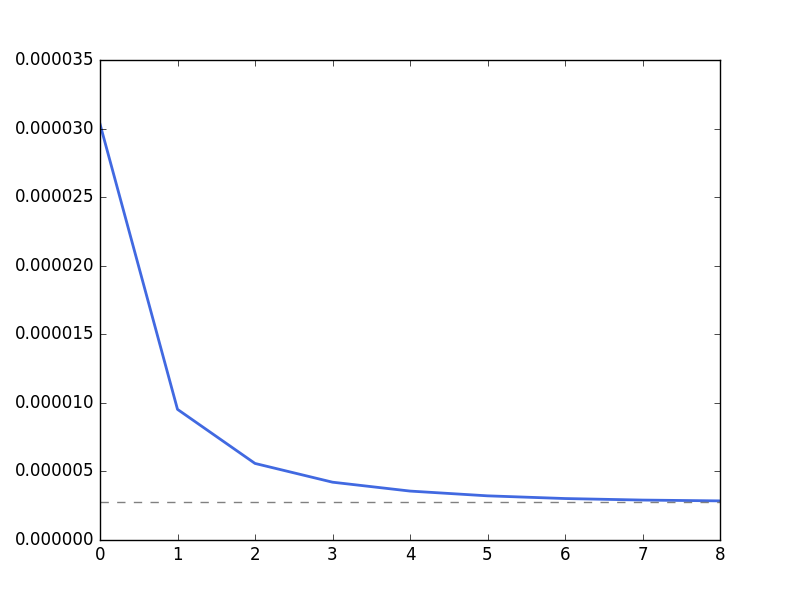
\includegraphics[scale=0.5]{t_order} \\
\newpage
\subsection{Иллюстрация решения}
\begin{figure}[!htb]
\minipage{0.32\textwidth}
  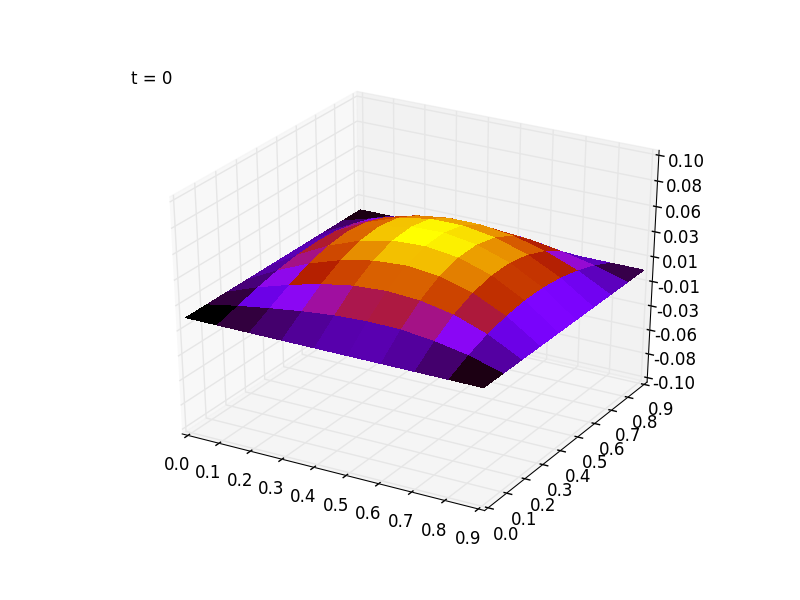
\includegraphics[width=\linewidth]{0}
\endminipage\hfill
\minipage{0.32\textwidth}
  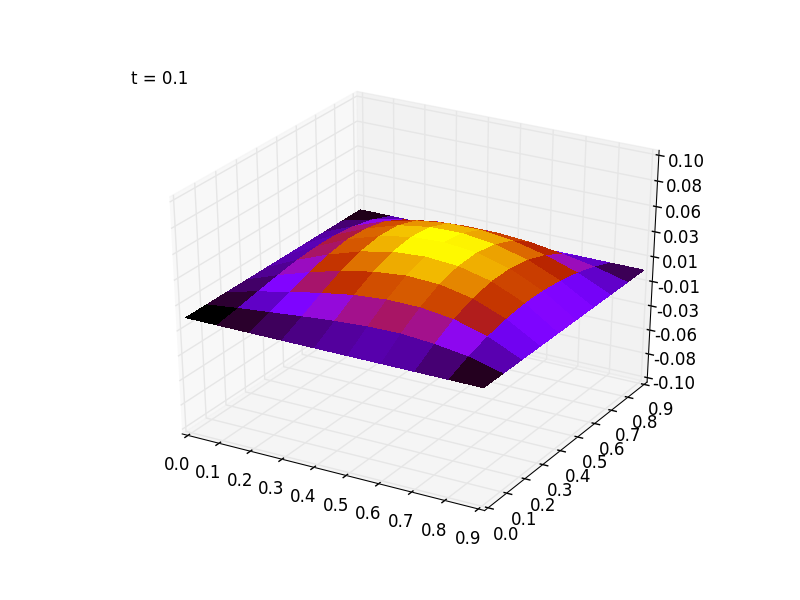
\includegraphics[width=\linewidth]{1}
\endminipage\hfill
\minipage{0.32\textwidth}%
  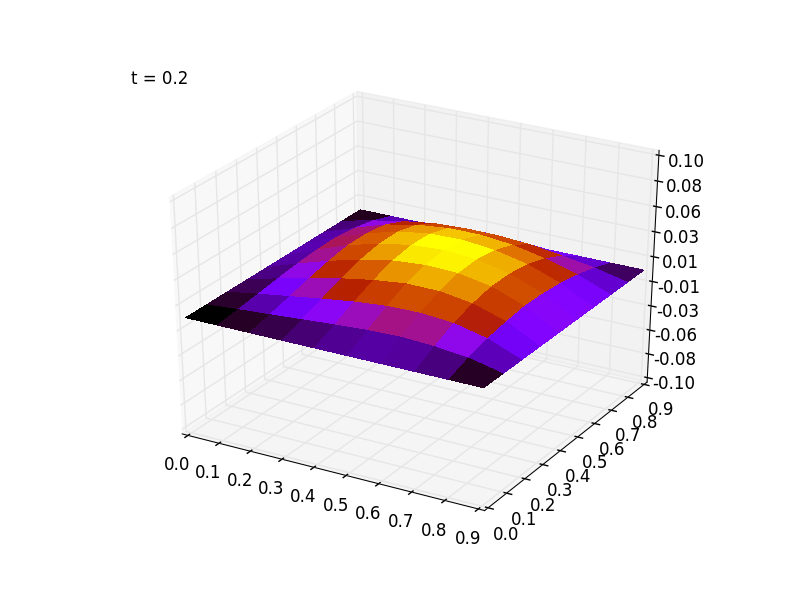
\includegraphics[width=\linewidth]{2}
\endminipage
\end{figure}
\begin{figure}[!htb]
\minipage{0.32\textwidth}
  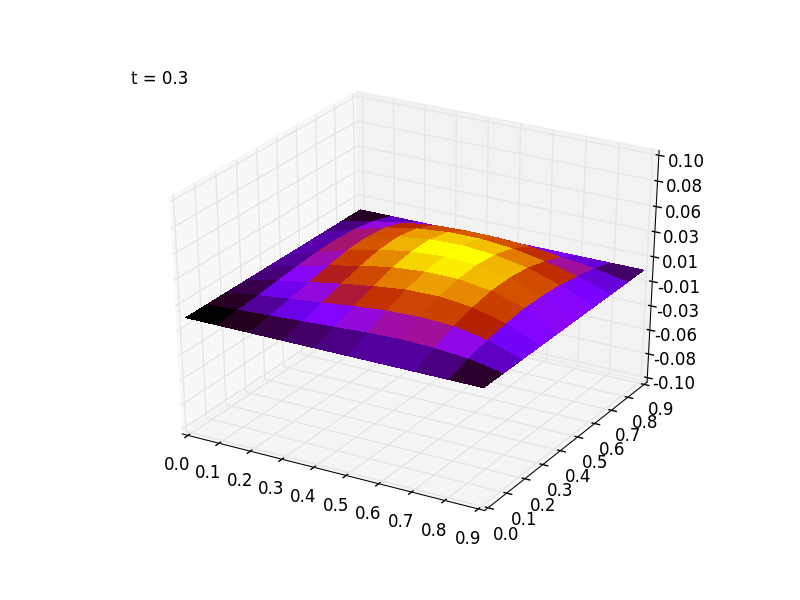
\includegraphics[width=\linewidth]{3}
\endminipage\hfill
\minipage{0.32\textwidth}
  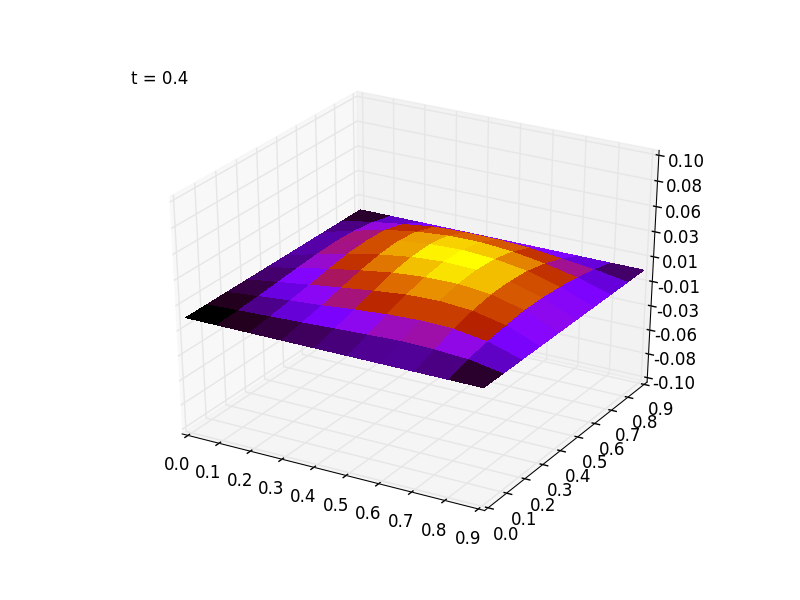
\includegraphics[width=\linewidth]{4}
\endminipage\hfill
\minipage{0.32\textwidth}%
  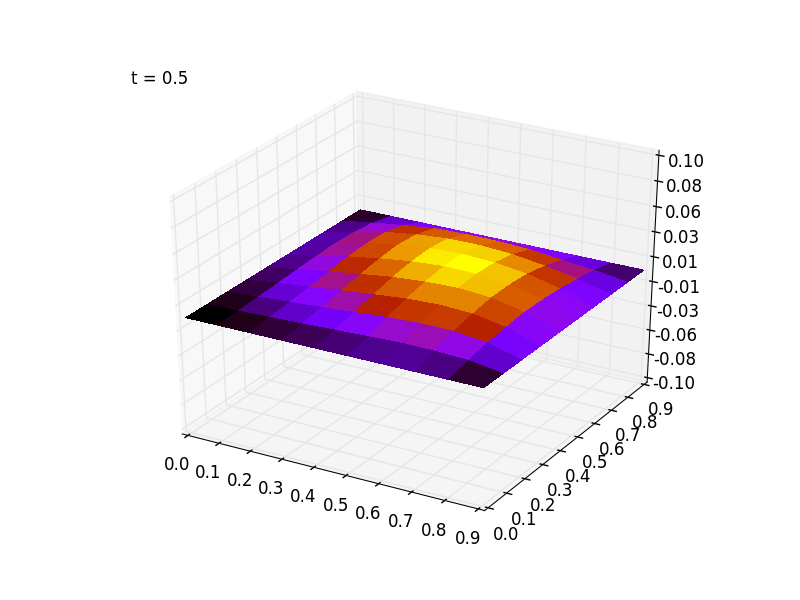
\includegraphics[width=\linewidth]{5}
\endminipage
\end{figure}
\begin{figure}[!htb]
\minipage{0.32\textwidth}
  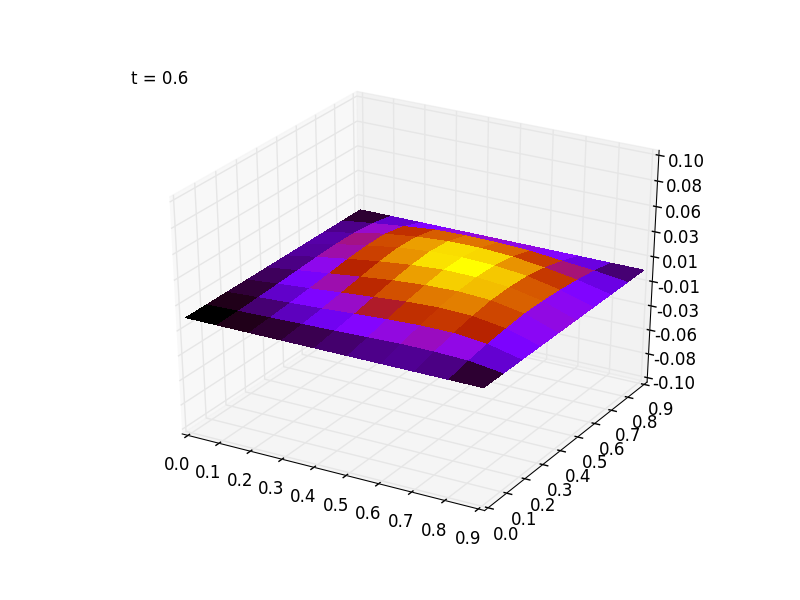
\includegraphics[width=\linewidth]{6}
\endminipage\hfill
\minipage{0.32\textwidth}
  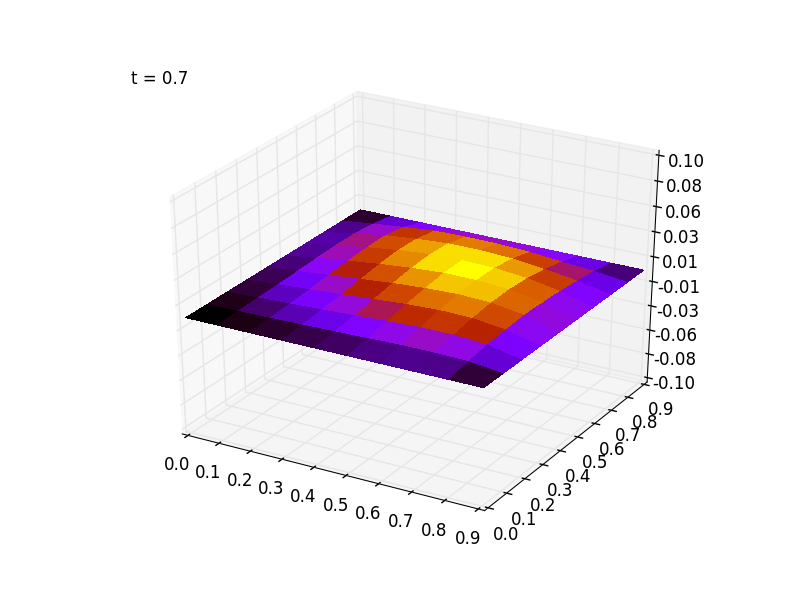
\includegraphics[width=\linewidth]{7}
\endminipage\hfill
\minipage{0.32\textwidth}%
  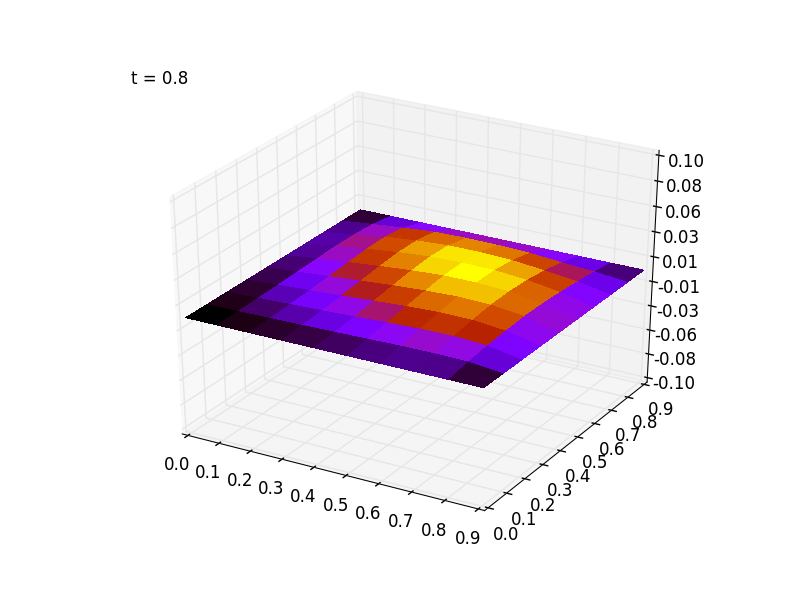
\includegraphics[width=\linewidth]{8}
\endminipage
\end{figure}
\end{document}
